\documentclass[12pt]{article}

%packages
\usepackage{fancyhdr}
\usepackage[margin=1in]{geometry}
\usepackage[utf8]{inputenc}
\usepackage{listings}
\usepackage{booktabs}
\usepackage{enumitem}
\usepackage{pdfpages}
\usepackage{graphicx}
\usepackage{xcolor}
\usepackage{rotating}
\usepackage{subcaption}
\usepackage{float}
\usepackage{amsmath}

%fancyheadr fix
\setlength{\headheight}{15pt}

%commands to lslistings
\lstset{
    basicstyle=\ttfamily\small,
    breaklines=true,     
    breakatwhitespace=true,
    frame=single,
    numbers=left,
    numberstyle=\tiny,
    columns=fullflexible,
    keepspaces=true
}


%title info
\newcommand{\doctitle}{STA 5635 HW 13}
\newcommand{\name}{Palmer Swanson}
\newcommand{\docdate}{\today}

%document
\begin{document}

\begin{center}
    {\Large \doctitle}\\[6pt]
    {\name}\\[3pt]
    {\docdate}
\end{center}
%\vspace{12pt}

%question 1
\section*{Part a}

\begin{figure}[htbp]
    \centering
    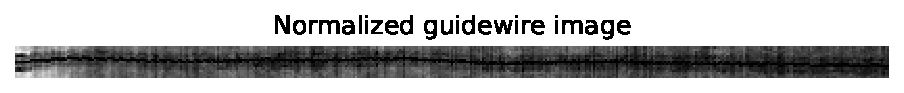
\includegraphics[width=1.0\textwidth]{../figures/normalized_image.pdf}
    \caption{Normalized Image with Guidewire almost horizontal}
    \label{fig:norm_image_guide}
\end{figure}

\begin{figure}[htbp]
    \centering
    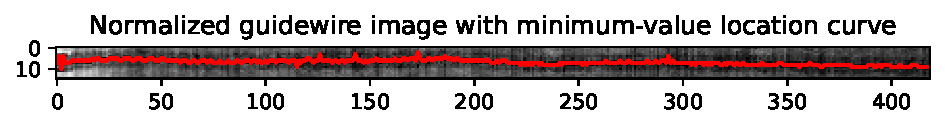
\includegraphics[width=1.0\textwidth]{../figures/gw_with_curve.pdf}
    \caption{Normalized Image with Minimum Value locations in each column of the image overlaid}
    \label{fig:norm_image_min_values}
\end{figure}

\section*{Part b}
Based upon what we have learned in class, I started by going through what algorithms could NOT work here.  
Decision trees and random forests don't make sense; they are supervised learning.  Logistic regression (classification)
doesn't work either.  Neural networks neither.  We aren't clustering, so PCA isn't appropiate.  Metric learning is close,
but isn't exactly what I'm looking for.  

There is a effectively a penalty term involved, but its not penalized loss functions as we learned them.  Yesterday, 
Prof. Barbu talked about using the Viterbi algorithm, and I realized that it can be thought of as a Hidden Markov Model,
estimated with the Viterbi algorithm.  My reasoning for this is that we can view the rows of the iamge as states, the 
columns as observations, \(I(c,i)\) as the emission cost, and the penalty term involving alpha acting as a transition cost.

\section*{Part c}
\begin{center}
\input{../output/results_table.tex}
\end{center}

\newpage
\section*{Part d}
\begin{figure}[htbp]
    \centering
    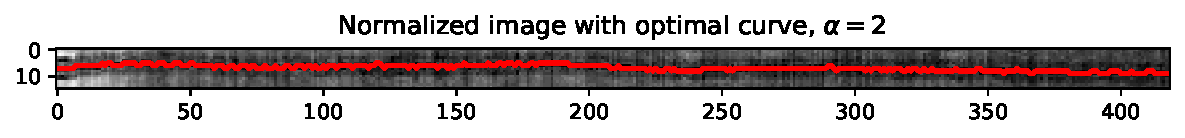
\includegraphics[width=1.0\textwidth]{../figures/gw_curve_alpha_2.pdf}
    \caption{Normalized Image with Approximation of Guidewire \(c\), \(\alpha=2\)}
    \label{fig:norm_image_alpha_2}
\end{figure}

\begin{figure}[htbp]
    \centering
    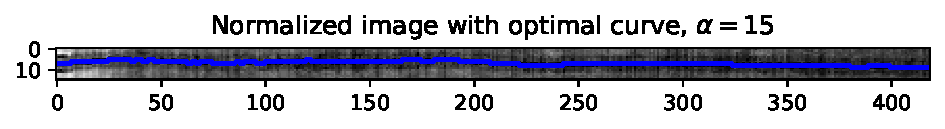
\includegraphics[width=1.0\textwidth]{../figures/gw_curve_alpha_15.pdf}
    \caption{Normalized Image with Approximation of Guidewire \(c\), \(\alpha=15\)}
    \label{fig:norm_image_alpha_15}
\end{figure}

\newpage
\newpage
%adding code
\appendix
\section*{Code}
\lstinputlisting[language=Python]{../code/hw13.py}

\end{document}